\documentclass[a4paper,12pt,obeyspaces,spaces,hyphens]{article}

\usepackage{agenda}
\usepackage{colortbl}
\usepackage{xcolor}
\usepackage{palatino}
\usepackage{calc}

\hypersetup{pdftitle={Embedded Linux kernel and driver development training},
  pdfauthor={Free Electrons}}

\begin{document}

\thispagestyle{fancy}

\setlength{\arrayrulewidth}{0.8pt}

\begin{center}
\LARGE
Embedded Linux kernel and driver development training\\
\large
5 days session
\end{center}
\vspace{1cm}

\small
\newcolumntype{g}{>{\columncolor{fedarkblue}}m{4cm}}
\newcolumntype{h}{>{\columncolor{felightblue}}X}

\arrayrulecolor{lightgray} {
  \setlist[1]{itemsep=-5pt}
  \begin{tabularx}{\textwidth}{|g|h|}
    {\bf Title} & Embedded Linux kernel and driver development
    training \\
    \hline

    {\bf Overview} &
    Understanding the Linux kernel \par
    Developing Linux device drivers \par
    Linux kernel debugging \par
    Porting the Linux kernel \par
    Working with the kernel development community \par
    Practical labs with the ARM-based Beagle Bone Black.\\
    \hline

    {\bf Duration} & {\bf Five} days - 40 hours (8 hours per day).
    \newline 50\% of lectures, 50\% of practical labs. \\
    \hline

    {\bf Trainer} & One of the engineers listed on
    \newline \url{http://free-electrons.com/training/trainers/}\\
    \hline

    {\bf Language} & Oral lectures: English or French.
    \newline Materials: English.\\
    \hline

    {\bf Audience} & People developing devices using the Linux kernel
    \newline People supporting embedded Linux system developers. \\
    \hline

    {\bf Prerequisites} & {\bf Knowledge and practice of Unix or
      GNU/Linux commands}
    \newline People lacking experience on this topic should get
    trained by themselves with our freely available on-line slides
    (\url{http://free-electrons.com/docs/command-line/})
    \newline {\bf Knowledge and practice of C programming} \\
    \hline

    {\bf Required equipment} &
    \begin{itemize}
    \item Video projector
    \item PC computers with at least 2 GB of RAM, and Ubuntu Linux
    installed in a {\bf free partition of at least 20 GB. Using Linux
      in a virtual machine is not supported}, because of issues
    connecting to real hardware.
    \item We need Ubuntu Desktop 12.04 (32 or 64 bit, Xubuntu and
    Kubuntu variants are fine). We don't support other
    distributions, because we can't test all possible package versions.
    \item {\bf Connection to the Internet} (direct or through the
    company proxy).
    \item {\bf PC computers with valuable data must be backed up}
    before being used in our sessions.  Some people have already made
    mistakes during our sessions and damaged work data.
    \end{itemize} \\
    \hline

    {\bf Materials} & Print and electronic copies of presentations and
    labs.
    \newline Electronic copy of lab files.\\
    \hline

\end{tabularx}}
\normalsize

\feagendatwocolumn
{Hardware}
{
  The hardware platform used for the practical labs of this training
  session is a {\bf BeagleBone Black}, which features:

  \begin{itemize}
  \item An ARM AM335x processor from Texas Instruments (Cortex-A8
    based), 3D acceleration, etc.
  \item 512 MB of RAM
  \item 2 GB of on-board eMMC storage
  \item USB host and device
  \item HDMI output
  \item 2 x 46 pins headers, to access UARTs, SPI busses, I2C busses
    and more.
  \end{itemize}
}
{}
{
  \begin{center}
    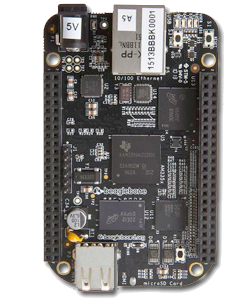
\includegraphics[height=5cm]{agenda/beagleboneblack.png}
  \end{center}
}

\feagendaonecolumn
{Labs}
{
  The practical labs of this training session use the following
  hardware peripherals to illustrate the development of Linux device
  drivers:

  \begin{itemize}
  \item A Wii Nunchuk, which is connected over the I2C bus to the
    BeagleBoneBlack. Its driver will use the Linux {\em input}
    subsystem.
  \item An additional UART, which is memory-mapped, and will use the
    Linux {\em misc} subsystem.
  \end{itemize}

  While our explanations will be focused on specifically the Linux
  subsystems needed to implement those drivers, they will always be
  generic enough to convey the general design philosophy of the Linux
  kernel. The informations learnt will therefore apply beyond just
  I2C, input or memory-mapped devices.
}


\section{Day 1 - Morning}

\feagendaonecolumn
{Lecture - Introduction to the Linux kernel}
{
  \begin{itemize}
  \item Kernel features
  \item Understanding the development process.
  \item Legal constraints with device drivers.
  \item Kernel user interface (/proc and /sys)
  \item Userspace device drivers
  \end{itemize}
}
\\
\feagendatwocolumn
{Lecture - Kernel sources}
{
  \begin{itemize}
  \item Specifics of Linux kernel development
  \item Coding standards
  \item Retrieving Linux kernel sources
  \item Tour of the Linux kernel sources
  \item Kernel source code browsers: cscope, Kscope, Linux Cross
    Reference (LXR)
  \end{itemize}
}
{Lab - Kernel sources}
{
  \begin{itemize}
  \item Making searches in the Linux kernel sources: looking for C
    definitions, for definitions of kernel configuration parameters,
    and for other kinds of information.
  \item Using the Unix command line and then kernel source code
    browsers.
 \end{itemize}
}

\section{Day 1 - Afternoon}
\feagendaonecolumn
{Lecture - Configuring, compiling and booting the Linux kernel}
{
  \begin{itemize}
  \item Kernel configuration.
  \item Native compiling. Generated files.
  \item Booting the kernel. Kernel booting parameters.
  \end{itemize}
}
\\
\feagendatwocolumn
{Lecture - NFS booting and cross-compiling}
{
  \begin{itemize}
  \item Booting on a directory on your GNU/Linux workstation, through
    NFS.
  \item Kernel cross-compiling
  \end{itemize}
}
{Lab - Kernel configuration, cross-compiling and booting on NFS}
{
  {\em Using the BeagleBoneBlack}
  \begin{itemize}
  \item Configuring, cross-compiling and booting a Linux kernel with
    NFS boot support.
  \end{itemize}
}
\\
\section{Day 2 - Morning}

\feagendatwocolumn
{Lecture - Linux kernel modules}
{
  \begin{itemize}
  \item Linux device drivers
  \item A simple module
  \item Programming constraints
  \item Loading, unloading modules
  \item Module parameters
  \item Module dependencies
  \item Adding sources to the kernel tree
  \item Generating patches to share them with others
  \end{itemize}
}
{Lab - Writing modules}
{
  {\em Continued from the previous lab}
  \begin{itemize}
  \item Write a kernel module with several capabilities, including
    module parameters.
  \item Access kernel internals from your module.
  \item Setup the environment to compile it
  \end{itemize}
}
\\
\feagendaonecolumn
{Lecture - Memory management}
{
  \begin{itemize}
  \item Linux: memory management - Physical and virtual (kernel and user) address spaces.
  \item Linux memory management implementation.
  \item Allocating with \code{kmalloc()}.
  \item Allocating by pages.
  \item Allocating with \code{vmalloc()}.
  \end{itemize}
}

\section{Day 2 - Afternoon}

\feagendatwocolumn
{Lecture - I/O memory and ports}
{
  \begin{itemize}
  \item I/O register and memory range registration.
  \item I/O register and memory access.
  \item Read / write memory barriers.
  \end{itemize}
}
{Lab - I/O memory and ports}
{
  \begin{itemize}
  \item Make a remote connection to your board through ssh.
  \item Access the system console through the network.
  \item Reserve the I/O memory addresses used by the serial port.
  \item Read device registers and write data to them, to send
    characters on the serial port.
  \end{itemize}
}
\\
\feagendatwocolumn
{Lecture - Character drivers}
{
  \begin{itemize}
  \item Device numbers
  \item Getting free device numbers
  \item Implementing file operations: read, write, open, close,
    ioctl...
  \item Exchanging data between kernelspace and userspace
  \item Character driver registration
  \end{itemize}
}
{Lab - Character drivers}
{
  {\em Using the BeagleBoneBlack}
  \begin{itemize}
  \item Writing a simple character driver, to write data to the serial port.
  \item On your workstation, checking that transmitted data is received correctly.
  \item Exchanging data between userspace and kernel space.
  \item Practicing with the character device driver API.
  \item Using kernel standard error codes.
  \end{itemize}
}

\section{Day 3 - Morning}

\feagendaonecolumn
{Lecture - Processes, scheduling, sleeping and interrupts}
{
  \begin{itemize}
  \item Process management in the Linux kernel.
  \item The Linux kernel scheduler and how processes sleep.
  \item Interrupt handling in device drivers: interrupt handler
    registration and programming, scheduling deferred work.
  \end{itemize}
}
\\
\feagendaonecolumn
{Lab - Sleeping and handling interrupts in a device driver}
{
  {\em Using the BeagleBoneBlack}
  \begin{itemize}
  \item Adding read capability to the character driver developed
    earlier.
  \item Register an interrupt handler.
  \item Waiting for data to be available in the read file operation.
  \item Waking up the code when data is available from the device.
  \end{itemize}
}

\section{Day 3 - Afternoon}

\feagendatwocolumn
{Lecture - Locking}
{
  \begin{itemize}
  \item Issues with concurrent access to resources
  \item Locking primitives: mutexes, semaphores, spinlocks.
  \item Atomic operations.
  \item Typical locking issues.
  \item Using the lock validator to identify the sources of locking
    problems.
  \end{itemize}
}
{Lab - Locking}
{
  {\em Continued from the previous lab}
  \begin{itemize}
  \item Observe problems due to concurrent accesses to the device.
  \item Add locking to the driver to fix these issues.
  \end{itemize}
}
\\
\feagendatwocolumn
{Lecture - Driver debugging techniques}
{
  \begin{itemize}
  \item Debugging with printk
  \item Proc and debugfs entries
  \item Analyzing a kernel oops
  \item Using kgdb, a kernel debugger
  \item Using the Magic SysRq commands
  \item Debugging through a JTAG probe
  \item SystemTap and demonstration
  \end{itemize}
}
{Lab - Investigating kernel faults}
{
 {\em Using the BeagleBoneBlack}
  \begin{itemize}
  \item Studying a broken driver.
  \item Analyzing a kernel fault and locating the problem in the
    source code.
  \end{itemize}
}
\section{Day 4 - Morning}

\feagendatwocolumn
{Lecture - mmap}
{
  \begin{itemize}
  \item Process virtual memory areas
  \item Maximizing performance with mmap, allowing applications to
    access the hardware directly.
  \item Implementing mmap in drivers
  \end{itemize}
}
{Lecture - The DMA API}
{
  \begin{itemize}
  \item The Linux kernel DMA API.
  \item Using it in device drivers.
  \end{itemize}
}
\\
\feagendaonecolumn
{Lecture - Kernel architecture for device drivers}
{
  \begin{itemize}
  \item Understand how the kernel is designed to support device
    drivers
  \item The kernel device driver ``framework'' for common types of
    devices
  \item The device model
  \item Binding devices and drivers
  \item Platform devices
  \item Interface in userspace: \code{/sys}
  \end{itemize}
}

\section{Day 4 - Afternoon}

\feagendatwocolumn
{Lecture - Serial drivers}
{
  \begin{itemize}
  \item As an illustration of one particular kernel framework, details
    on the serial driver framework.
  \end{itemize}
}
{Lab - Implement a serial driver}
{
  {\em Using the BeagleBoneBlack}
  \begin{itemize}
  \item Implement parts of a serial driver through the kernel's serial
    framework.
  \end{itemize}
}

\section{Day 5 - Morning}
\feagendaonecolumn
{Lecture - Kernel boot-up details}
{
  \begin{itemize}
  \item Detailed description of the kernel boot-up process, from
    execution by the bootloader to the execution of the first
    userspace program.
  \item Initcalls: how to register your own initialization routines.
  \end{itemize}
}
\\
\feagendatwocolumn
{Lecture - Porting the Linux kernel}
{
  \begin{itemize}
  \item Porting the Linux kernel. Creating board dependent code.
  \item Detail study of code for an ARM board.
  \end{itemize}
}
{Lecture - Lecture - Introduction to power management}
{
  \begin{itemize}
  \item Supporting frequency scaling
  \item CPU and board specific power management.
  \item Power management in device drivers.
  \item Control from user space.
  \item Saving power in the idle loop.
  \item Voltage and current regulator framework
  \item Studying power management implementations in the Linux kernel.
  \end{itemize}
}
\\
\feagendaonecolumn
{Lab - Power management}
{
  {\em Using the Linux workstation and if possible, the BeagleBoneBlack}
  \begin{itemize}
  \item Practicing with the standard power management interfaces:
    suspend / resume and cpu frequency control.
  \item Identifying top sources of power consumption with
    \code{PowerTop}.
  \end{itemize}
}

\section{Day 5 - Afternoon}
\feagendaonecolumn
{Lecture - Working with the community}
{
  \begin{itemize}
  \item How to get help from the community.
  \item Report bugs.
  \item Generate and send patches.
  \item Useful resources about the kernel
  \end{itemize}
}
\\
\feagendatwocolumn
{Lecture - Managing kernel sources with git}
{
  {\em Very useful to manage your changes to the Linux kernel
    (drivers, board support code), staying in sync with mainline
    updates.}
  \begin{itemize}
  \item Cloning an existing git tree
  \item Creating your own branch with your own changes.
  \item Generating patches against the reference tree.
  \item Review of useful git commands.
  \item Understanding the work flow used by kernel developers, through
    the study of typical scenarios.
  \end{itemize}
}
{Lab - Using git}
{
  \begin{itemize}
  \item Create your own git branch from the mainline tree.
  \item Get changes from trees and generate your own patchset.
  \item Keep your branch updated with the changes in your reference
    tree.
  \end{itemize}
}

 \end{document}

